\documentclass{article}
\usepackage{booktabs}
% ---------------------------------------------------------------------
%             FOR DRAFTING / REVIEW (DELETE BEFORE SUBMISSION)
% ---------------------------------------------------------------------
\usepackage{caption}
\usepackage{subcaption}
\usepackage[T1]{fontenc}
\usepackage[british]{babel}
\usepackage{microtype}
\usepackage[tt=false]{libertine}
\usepackage{xcolor}
\definecolor{blue}{RGB}{33,150,209}
\definecolor{red}{RGB}{255,0,0}
\usepackage{xurl}
\usepackage[colorlinks=true, allcolors=blue]{hyperref}
\usepackage{pdfpages}
\usepackage{enumitem}
\usepackage{lineno}
\usepackage{float}
\setlength{\linenumbersep}{5pt}
% Save the old \texttt command
\let\oldtexttt\texttt
% Redefine the \UrlFont to use a smaller typewriter font
\renewcommand{\UrlFont}{\ttfamily\small}
% Redefine the \texttt command to use a smaller font size and allow line breaks
\renewcommand{\texttt}[1]{{\ttfamily\small\nolinkurl{#1}}}

\usepackage{longtable}
% --------------------------------------------------------------------- %

\usepackage{tcolorbox}
\newcommand{\cbox}[1]{
    \begin{tcolorbox}[hbox, colback=red!5!white, colframe=red!65!black, boxrule=0.25pt, boxsep=2pt, left=2pt, right=2pt, top=1pt, bottom=1pt]
        \small\sffamily #1
    \end{tcolorbox}
}

% \usepackage{graphicx}
\usepackage[margins=1cm]{geometry}


\begin{document}

\title{Supplementary Material for the T-reX Tool}
\author{Stewart Charles McDowall, Elizabeth Lanphear, Carlos Felipe Rocha Blanco, Stefano Cucurachi}
\date{\today}

\maketitle

\section{Metadata of the T-reX tool}

\begin{table}[h]
    \caption{T-reX tool metadata}\label{tab:metadata}
    \centering
    \begin{tabular}{ll}
    \toprule
    \textbf{Item} & \textbf{Details} \\
    \midrule
    Current version & 0.1.21 \\
    DOI & \url{zenodo.org/doi/10.5281/zenodo.10431180} \\
    Code repository & \url{github.com/Stew-McD/T-reX} \\
    License & CC0--1.0 license \\
    Versioning system & git \\
    Language & Python \\
    Documentation & \url{T-reX.readthedocs.io} \\
    Main dependencies & brightway2, premise, wurst \\
    \bottomrule
    \end{tabular}
\end{table}

\section{List of modules in the T-reX python package}

\subsection{Functional modules}
\begin{itemize}
    \item \texttt{future\_scenarios}: Creates prospective LCA databases based on future scenarios.
    \item \texttt{explode\_database}: Responsible for expanding a Brightway2 database into detailed exchange lists.
    \item \texttt{search\_waste}: Provides functions for searching and categorising waste generation-related exchange data.
    \item \texttt{search\_material}: Provides functions for searching and categorising material demand-related exchange data.
    \item \texttt{make\_custom\_database}: Facilitates the creation of custom databases based on the waste and material search categories.
    \item \texttt{method\_editor}: Manages the custom LCIA methods for waste and material footprint calculations.
    \item \texttt{exchange\_editor}: Appends `pseudo-biosphere' exchanges to activities to match their waste generation and material demand exchanges in the technosphere.
    \item \texttt{verify\_database}: Performs verification of the manipulated databases.
\end{itemize}

\subsection{Configuration modules}
\begin{itemize}
    \item \texttt{custom\_config}: Provides functions for managing the configuration of the T-reX package.
    \item \texttt{user\_settings}: The main configuration file, for defining the project and database settings (user editable).
    \item \texttt{queries\_waste}: Defines search parameters and categories for waste generation exchanges (user editable).
    \item \texttt{queries\_materials}: Defines search parameters and categories for material demand exchanges (user editable).
\end{itemize}

\section{Flowchart of the T-reX tool}

% \autoref{fig:flowchart} shows the computation flowchart of the T-reX tool.

\begin{figure}
    \centering
    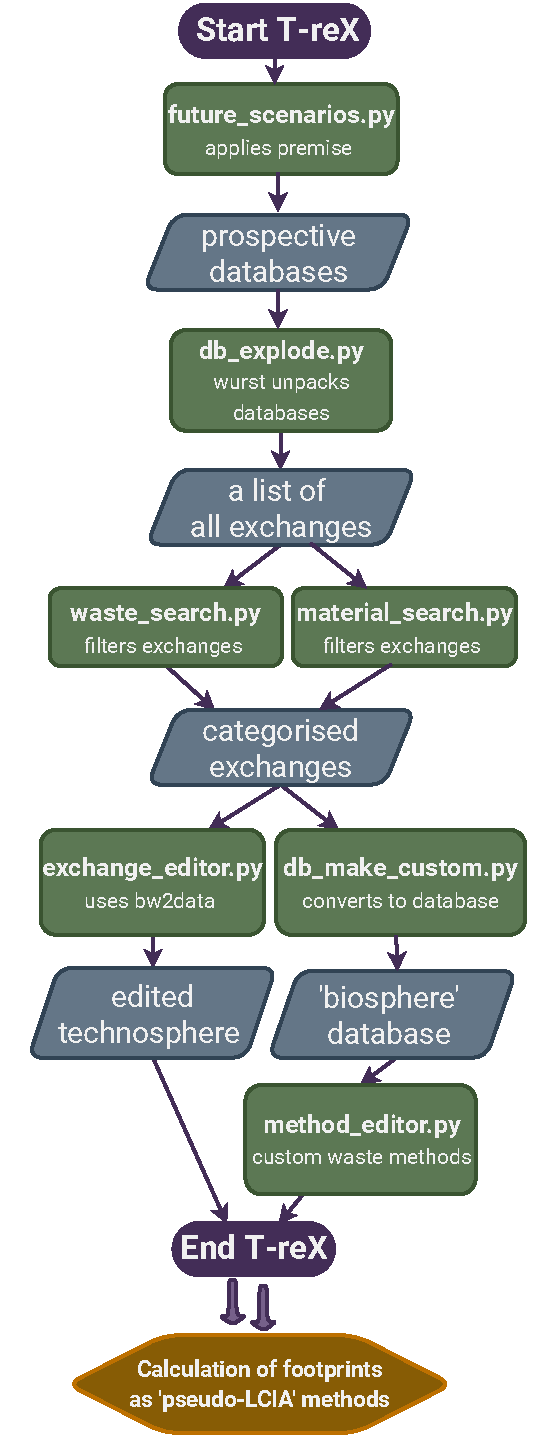
\includegraphics[height=0.8\textheight]{figures/T-reX_flowchart.pdf}
    \caption{Computational flowchart of the T-reX tool}\label{fig:flowchart}
\end{figure}


\section{List of Materials and Their Markets}

\begin{longtable}{ll}
    \caption{A comprehensive list of various materials in the default configuration.} \label{tab:materials} \\
    \toprule
    \textbf{Market Name} & \textbf{Material group} \\
    \midrule
    \endfirsthead
    \multicolumn{2}{c}%
    {\tablename\ \thetable\ -- \textit{Continued from previous page}} \\
    \toprule
    \textbf{Market Name} & \textbf{Material group} \\
    \midrule
    \endhead
    \midrule \multicolumn{2}{r}{\textit{Continued on next page}} \\
    \endfoot
    \bottomrule
    \endlastfoot

market for aluminium & aluminium \\
market for antimony & antimony \\
market for bauxite & bauxite \\
market for beryllium & beryllium \\
market for bismuth & bismuth \\
market for cadmium & cadmium \\
market for calcium borates & borates \\
market for cement & cement \\
market for cerium & cerium \\
market for chromium & chromium \\
market for coal & coal \\
market for cobalt & cobalt \\
market for coke & coke \\
market for copper & copper \\
market for dysprosium & dysprosium \\
market for erbium & erbium \\
market for europium & europium \\
market for electricity & electricity \\
market for ferroniobium & niobium \\
market for fluorspar & fluorspar \\
market for gadolinium & gadolinium \\
market for gallium & gallium \\
market for gold & gold \\
market for graphite & graphite \\
market for hafnium & hafnium \\
market for helium & helium \\
market for holmium & holmium \\
market for hydrogen & hydrogen \\
market for indium & indium \\
market for latex & latex \\
market for lithium & lithium \\
market for magnesium & magnesium \\
market for natural gas & natural gas \\
market for nickel & nickel \\
market for palladium & palladium \\
market for petroleum & petroleum \\
market for phosphate & phosphate rock \\
market for platinum & platinum \\
market for rare earth & rare earth \\
market for rhodium & rhodium \\
market for sand & sand \\
market for selenium & selenium \\
market for scandium & scandium \\
market for silicon & silicon \\
market for silver & silver \\
market for sodium borates & borates \\
market for strontium & strontium \\
market for tantalum & tantalum \\
market for tellurium & tellurium \\
market for tin & tin \\
market for titanium & titanium \\
market for uranium & uranium \\
market for tungsten & tungsten \\
market for vanadium & vanadium \\
market for vegetable oil & vegetable oil \\
market for tap water & water \\
market for water & water \\
market for zinc & zinc \\
market for zirconium & zirconium \\
\bottomrule
\end{longtable}

\end{document}